%%%%%%%%%%%%%%%%%%%%%%%%%%%%%%%%%%%%%%%%%%%%%%%%%%%%%%%%%%%
%                       EXPOSITION DU SUJET               %
%%%%%%%%%%%%%%%%%%%%%%%%%%%%%%%%%%%%%%%%%%%%%%%%%%%%%%%%%%%

Le traitement d'images est un ensemble de méthodes permettant d'étudier et de transformer une ou plusieurs images à l'aide de moyens mathématiques et numériques. Le principe du traitement d'images consiste à extraire certaines informations de celles-ci, afin de les étudier ou de les modifier.Il est utilisé dans beaucoup d'applications telles que l'amélioration du contraste, l'application d'un filtre(flou, lissage, changement de couleurs), ou encore les détections et identifications d'objets par exemple. 

Aujourd'hui, nous nous intéressons à l'incrustation d'images. A partir de deux images, comment sélectionner une partie de la première et l'incruster de la manière la plus naturelle possible dans la seconde ? 
\newline
Afin d'éclaircir nos propos et d'identifier les problèmes que nous devons résoudre, voici un exemple de ce que nous souhaitons faire.\newline
Nous disposons des deux images présentées ci-dessous, l'image T(arget) et l'image S(ource). 
\newline
\begin{figure}[!htb]
   \begin{minipage}{0.48\textwidth}
     \centering
     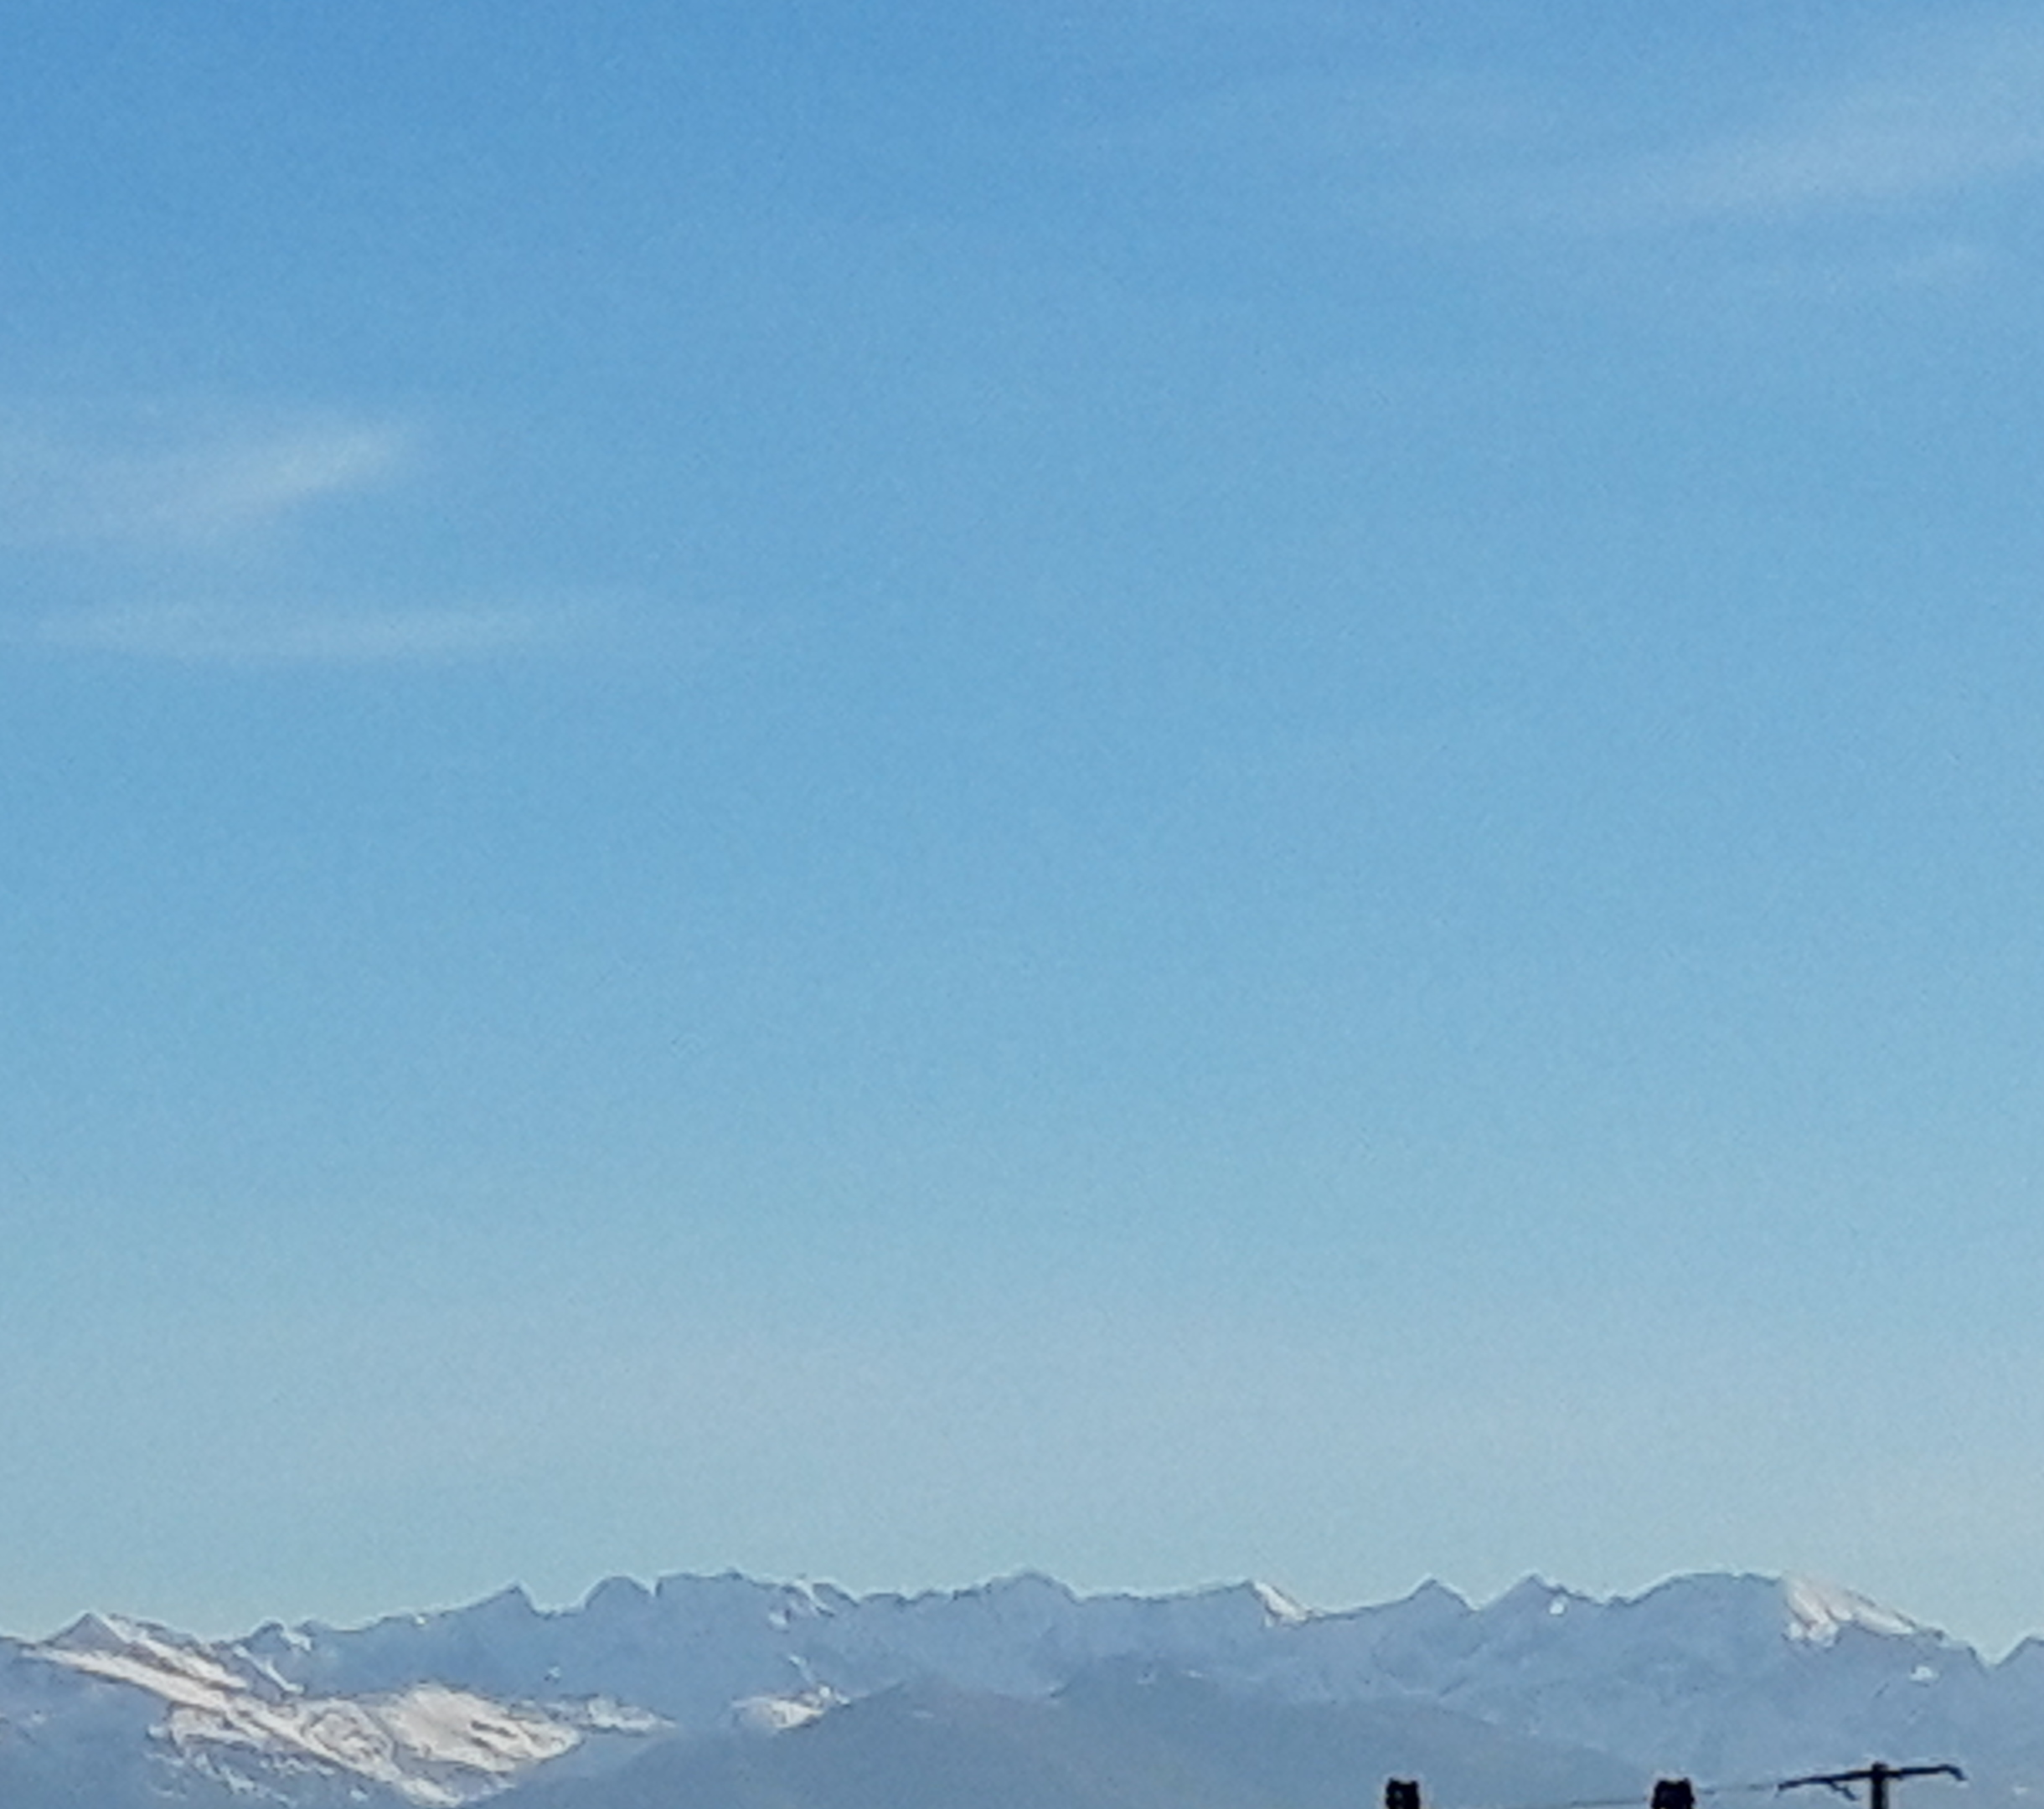
\includegraphics[width = 150pt]{Images/Montagne.jpg}
     \caption{Image T}
      \end{minipage}\hfill
   \begin{minipage}{0.48\textwidth}
     \centering
     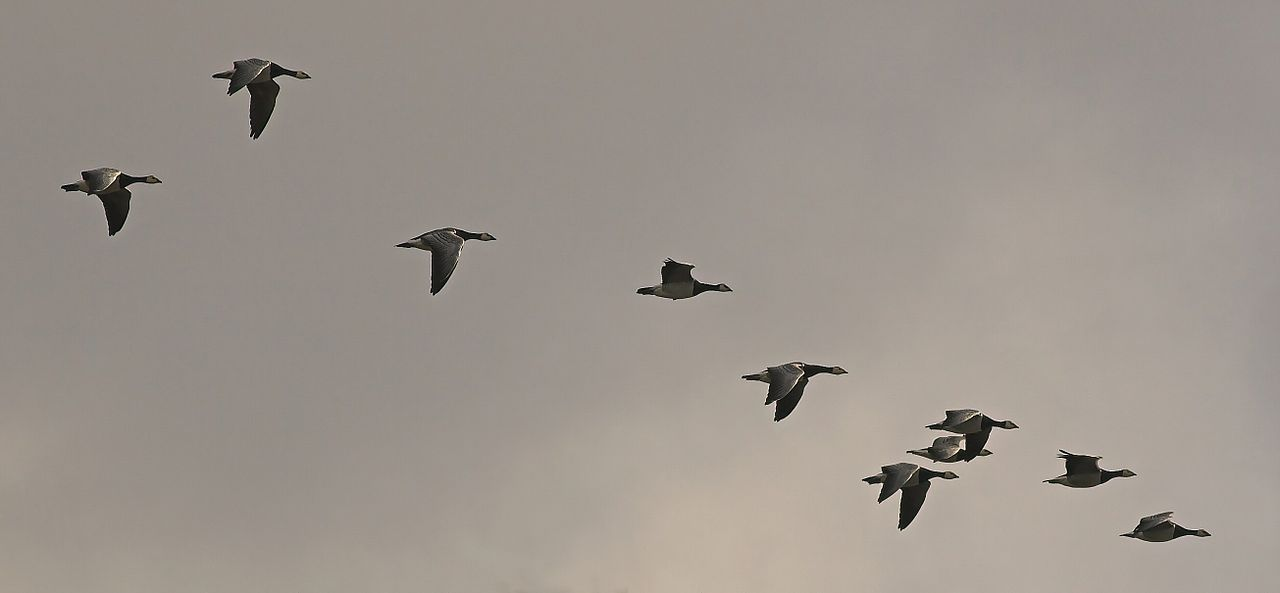
\includegraphics[width= 150pt]{Images/Oiseau.jpg}
     \caption{Image S}\label{Fig:Data2}
   \end{minipage}
\end{figure}

L'objectif est d'incruster toute ou partie de l'image S dans l'image T. En terme de manipulations, cela consiste à effectuer un copier/coller ou encore un clônage de la seconde image dans la première.
Le résultat que nous attendons pour une incrustation "réussie" est un résultat comme celui présenté ci-dessous : 
    
\begin{center}
\begin{figure}[!htb]
   \centering
     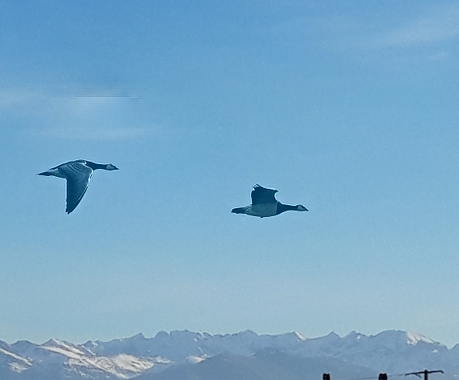
\includegraphics[width = 150pt]{Images/clonage_done.png}
     \caption{Image  finale attendue}
\end{figure}
\end{center}
Cette image est extraite d'une simulation effectuée sur 'ipol.im/...'.Nous comparerons nos images obtenues avec celle-ci à la fin de ce rapport.\newline
Ce résultat semble naturel, les marques et bords de l'image qui a été collée sont très peu visibles, les oiseaux semblent faire partie de l'image finale.
Mais comment obtenir un tel résultat ? 
\newline
Reprenons nos deux images séparées, T et S. Commençons par effectuer un simple copier/coller. Pour faire cela, il suffit de prendre une partie de l'image S,  puis de la transférer à l'endroit voulu dans l'image T. En effectuant cette manipulation voici l'image que nous devrions obtenir : 
\begin{center}
\begin{figure}[H]
     \centering
     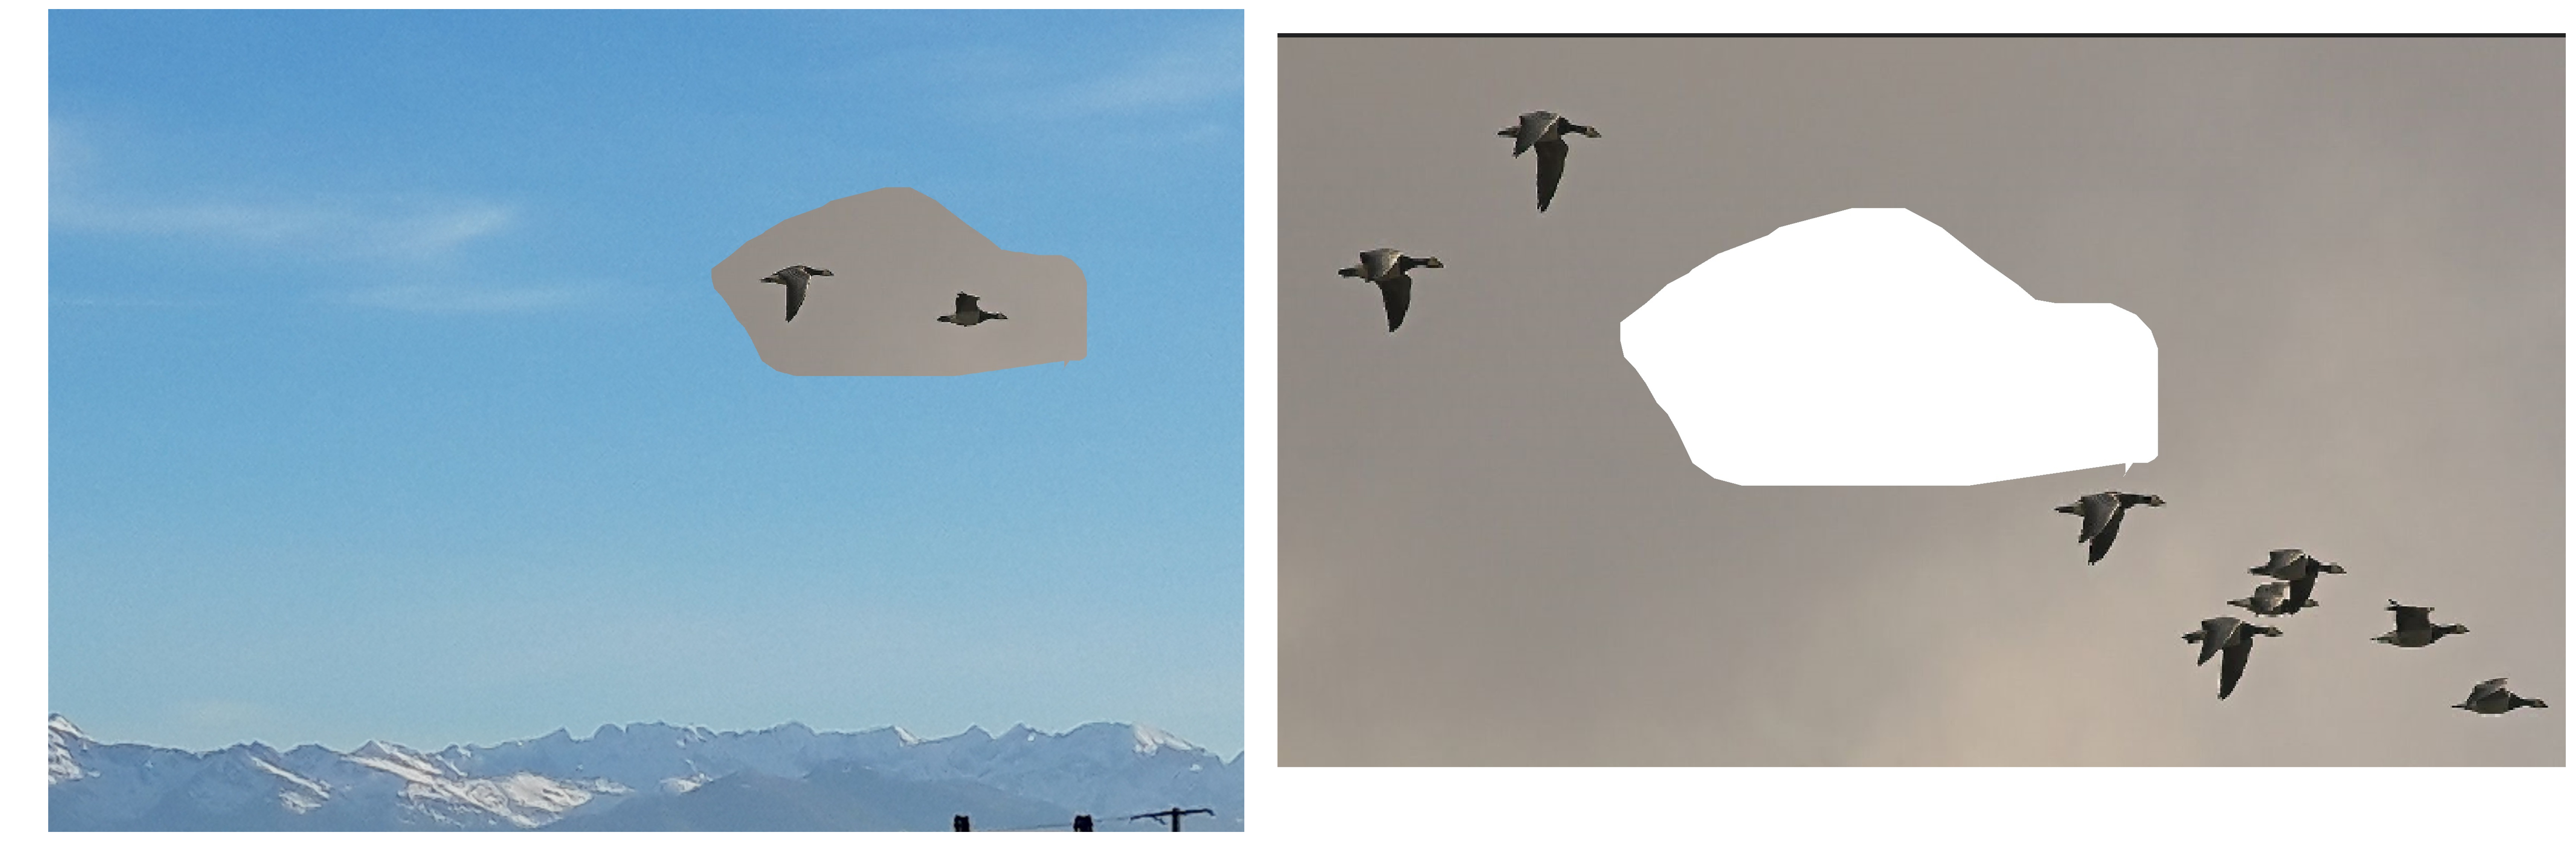
\includegraphics[width = 200pt]{Images/collage1.jpg}
     \caption{Simple copier/coller}
\end{figure}
\end{center}

Ce résultat n'est bien entendu pas convenable et bien loin de l'image finale attendue. Le découpage et la démarcation entre image originale et image collée sont beaucoup trop visibles, les couleurs ne sont pas les mêmes et incohérentes. Nous souhaitons obtenir un résultat beaucoup plus naturel, comme écrit plus haut. Cette simple manipulation n'est donc pas suffisante pour effectuer le clônage cohérent d'une image dans une autre. \newline

Il semble donc évident de vouloir modifier l'image finale obtenue afin qu'elle paraisse la plus naturelle possible. Nous verrons tout au long de ce rapport, quels sont les changements a effectuer, et comment la résolution d'une équation aux dérivées partielles, nous permet d'obtenir un bien meilleur résultat. 

%%%%%%%%%%%%%%%%%%%%%%%%%%%%%%%%%%%%%%%%%%%%%%%%%%%%%%%%%%
%           TRADUCTION SOUS FORMES MATHEMATIQUES         %
%%%%%%%%%%%%%%%%%%%%%%%%%%%%%%%%%%%%%%%%%%%%%%%%%%%%%%%%%%

\subsection{Traduction du problème sous formes mathématiques.}

Comme écrit plus haut nous souhaitons apporter des modifications au précédent collage afin qu'il corresponde au mieux à nos attentes. Pour ce faire, considérons I, la partie de l'image finale à modifier. Nous pouvons ainsi représenter le problème sous forme schématique. 
\begin{center}
    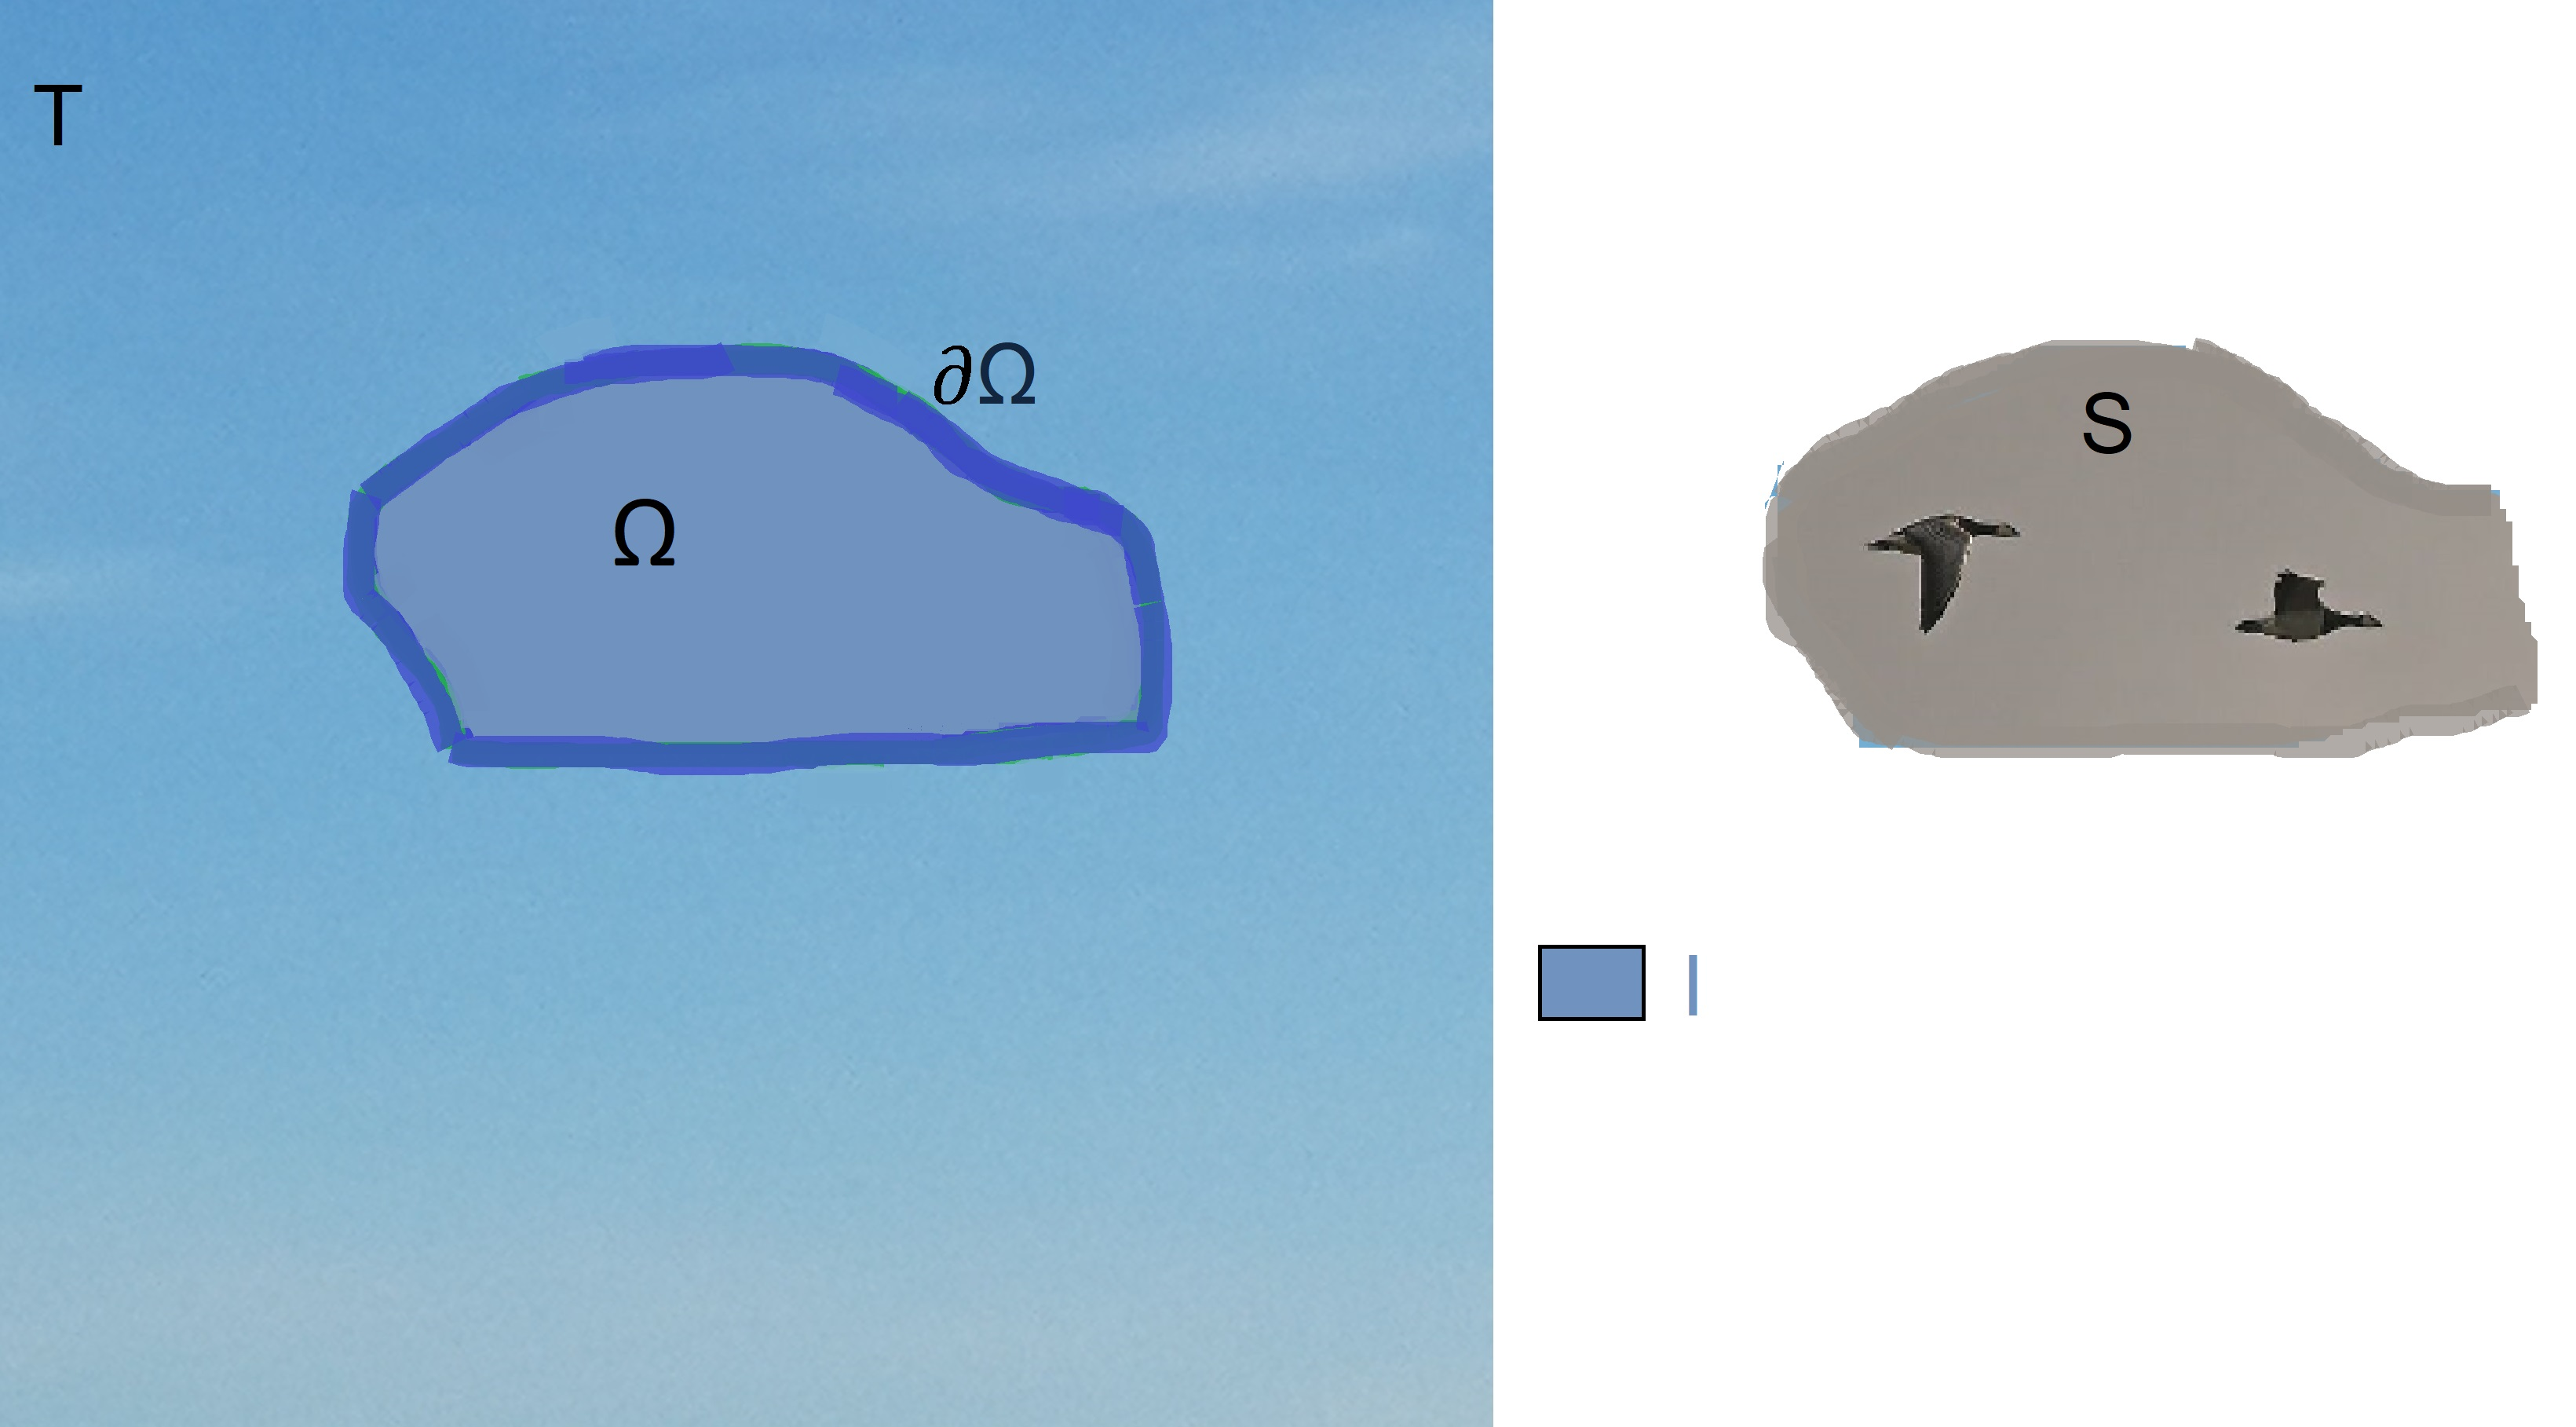
\includegraphics[width = 200pt]{Images/Schee.jpg}
\end{center}

Ici : 
\begin{itemize}
    \item T est l'image "Target", l'image destination, l'image sur laquelle s'effectuera le collage, l'arrière plan. 
    \item S est l'image "Source", l'image que nous souhaitons coller.
    \item $\Omega$ est le domaine dans lequel se trouvent nos inconnues.
    \item $\partial \Omega$ est la frontière de $\Omega$.
    \item I est notre inconnue, la partie de l'image que nous ne connaissons pas et que nous voulons remplir.
\end{itemize}

Nous souhaitons en effet, trouver une fonction I qui satisfasse un certain nombre de critères, afin de correspondre au résultat voulu.  
IL faut donc déterminer la fonction $I$.Cette fonction représente notre image modifiée. Mais quelles sont les conditions qu'elle doit remplir pour que le rendu soit le meilleur possible? Notre nouvelle image I doit-elle être plus proche de l'image collée S, ou de l'image d'arrière-plan T ? \newline
Pour répondre à cette question, reprenons le problème de départ. \newline

Pour que l'image obtenue paraisse naturelle,il faut que l'image obtenue dénature le moins possible les deux images sélectionnées au départ. En effet, nous devons garder les détails de l'image collée S, ne pas modifier les variations qu'elle pourrait posséder comme les contours des objets lui appartenant, par exemple.Nous devons pouvoir retrouver les informations présentes dans celle-ci. Il faut donc que les variations présentes dans $I$ soient presque identiques à celles de S. Mathématiquement, cela est équivalent à dire que les gradients de $I$ et S soient très proches, voir identiques. Donc à résoudre cette équation :
\begin{center}
    $$ min \iint_\Omega || \nabla I_{x,y} - \nabla S_{x,y}||^2 dxdy$$
\end{center} 

Mais les démarcations entre l'image collée  et l'image d'arrière-plan T, ne doivent pas non plus être visibles, il faut donc que les pixels se situant sur cette partie là, i.e $\partial \Omega$, soient le plus proches possible de T .  Nous voulons donc, mathématiquement, chercher : 
\begin{center}
    $I_{(x,y)} = T_{x,y} \ sur\ \partial \Omega$
\end{center}

Répondre au problème implique donc de résoudre un problème variationnel classique auquel des conditions sur le bord de Dirichlet sont ajoutées. 
Réécrivons le problème mathématique que nous cherchons à résoudre :  

\begin{center}
\begin{equation*}
\left\{
\begin{aligned}
 min \iint_\Omega || \nabla I_{x,y} - \nabla S_{x,y}||^2 dxdy\\
 I_{(x,y)} = T_{x,y} \ sur\ \partial \Omega
\end{aligned}
\right.
\end{equation*}
\end{center}


\subsection{Résolution dans le cas discret}
Notons $g(\nabla f, v)$ la fonction  : 
$$g(\nabla f, v) =\int ||\nabla f-v ||^2$$ 
\newline
Rappelons qu'ici $\nabla f$ est le gradient de f que l'on peut noter $\nabla f = (\frac{\partial f}{\partial x} \frac{\partial f}{\partial y})^T$ et v est un vecteur que l'on notera $v = (v_x, v_y)$. 
Ainsi nous pouvons réecrire g sous la forme suivante : 
$$g(\nabla f, v) =\int( (\frac{\partial f}{\partial x}-v_x)^2+(\frac{\partial f}{\partial y}-v_y)^2) $$\newline

Mais la fonction f qui minimise le problème posé,  satisfait l'équation d'Euler-Lagrange ci-dessous : 

\begin{equation*}
    \frac{\partial g}{\partial f}-\frac{d}{dx}\frac{\partial g}{\partial f   }-\frac{d}{dy}\frac{\partial g}{\partial f}= 0 \\
\end{equation*}
\begin{equation*}
    \frac{\partial g}{\partial f}-\frac{d}{dx}\frac{\partial g}{\partial f}-\frac{d}{dy}\frac{\partial g}{\partial f}= 0 \\
\end{equation*}

\begin{equation*}
    2\times()
\end{equation*}

\begin{center}
    
\includegraphics[width = 100pt]{Images/EXPLICATIONS_needed.png}
\end{center}

\begin{equation*}
    2(\frac{\partial^2 f}{\partial x^2}-\frac{\partial v_x}{\partial x}+\frac{\partial^2 f}{\partial y^2}\frac{\partial v_y}{\partial y}) = 0 ?
\end{equation*}

\begin{equation}
    \Delta f = div v
\end{equation}



Résoudre ce problème variationnel est équivalent à résoudre l'équation de poisson avec conditions aux bords de Dirichlet, suivante :
\begin{center}
    \begin{equation*}
        \left\{
        \begin{aligned}
         \Delta I = \Delta S  \ sur \  \Omega \\
          I = T \ sur \  \partial \Omega
        \end{aligned}
        \right.
    \end{equation*}
\end{center}

Nous verrons deux approches afin de résoudre cette équation, la première utilisant des discrétisations, la seconde la méthode de Fourier. 

